\documentclass[10pt]{jsarticle}

%% パッケージ
\usepackage{titlesec} % sectionの見た目を編集
\usepackage{color} % 文字・背景の色を編集
\usepackage{url} % URLを出力
\usepackage{amsmath,amssymb} % 数式全般
\usepackage{mathtools}
\usepackage[dvipdfmx]{graphicx} % 図の挿入
\usepackage{pgfplots}
\usepackage{tikz} % 図の描画
\usetikzlibrary{intersections,calc,arrows.meta} % TikZのライブラリを追加

%% sectionの修飾
% 四角+下線
\titleformat{\part}[block]
{}{}{0pt}
{
  \colorbox{black}{\begin{picture}(0,10)\end{picture}}
  \hspace{0pt}
  \normalfont \Large\bfseries
  \hspace{-4pt}
}
[
\begin{picture}(100,0)
  \put(3,18){\color{black}\line(1,0){300}}
\end{picture}
\\
\vspace{-30pt}
]
\renewcommand{\thesection}{\textbf{問題\Roman{section}}}
\renewcommand{\thesubsection}{\textbf{問\arabic{subsection}}}
\renewcommand{\thesubsubsection}{\textbf{(\alph{subsubsection})}}


\setcounter{tocdepth}{3}
\begin{document}

\title{東北大学工学部編入学試験過去問解答}
\author{comimome \\ \url{https://github.com/comimome/}}
\date{\today}
\maketitle

\tableofcontents%目次
\newpage

\part{はじめに}

\newpage

\part{令和5年度 数学}


\section{}


\subsection{}

ベクトル $\overrightarrow{\mathrm{AB}}$ を求め,その大きさを計算する.$\overrightarrow{\mathrm{AB}}$ は

\begin{gather*}
  \overrightarrow{\mathrm{AB}} = \begin{pmatrix}4 \\ 5 \\ -2 \end{pmatrix} - \begin{pmatrix}2 \\ 3 \\ -1 \end{pmatrix} = \begin{pmatrix}2 \\ 2 \\ -1 \end{pmatrix}
\end{gather*}

となる.よって

\begin{gather*}
  \lvert\overrightarrow{\mathrm{AB}}\lvert = \sqrt{2^2 + 2^2 + (-1)^2} = \sqrt{9} = 3
\end{gather*}

である.


\subsection{}

\begin{tikzpicture}
  \coordinate (A) at (2,3,-1) node [below left] at (A) {A};
  \coordinate (B) at (4,5,-2) node [below right] at (B) {B};
  \draw [name path=AB][thick](A)--(B);
  \draw [name path=cir_A][thick](A) circle[radius=1];
  \draw [name path=cir_B][thick][dotted](B) circle[radius=3];
  \path [name intersections={of=AB and cir_A, by={C}}];
  \fill (C) node [above] {C};
  \foreach\P in {A,B,C} \fill[black](\P)circle(0.06);
\end{tikzpicture}

線分 $\mathrm{AB}$ と球面 $\mathrm{\alpha}$ の交点を $\mathrm{C}$ とおく.
球面 $\mathrm{\beta}$ が球面 $\mathrm{\alpha}$ と共有点を持つ条件は問1より以下のようになる.

\begin{gather*}
  \lvert\overrightarrow{\mathrm{AB}}\lvert + \lvert\overrightarrow{\mathrm{AC}}\lvert  \ge \mathrm{r} \ge \lvert\overrightarrow{\mathrm{AB}}\lvert - \lvert\overrightarrow{\mathrm{AC}}\lvert \\
  3 \ge \mathrm{r} \ge 2
\end{gather*}


\subsection{}

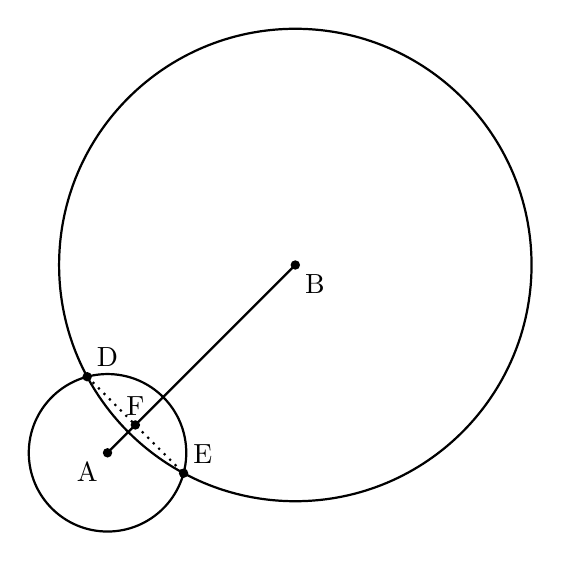
\begin{tikzpicture}
  \coordinate (A) at (2,3,-1) node [below left] at (A) {A};
  \coordinate (B) at (4,5,-2) node [below right] at (B) {B};
  \draw [name path=AB][thick](A)--(B);
  \draw [name path=cir_A][thick](A) circle[radius=1];
  \draw [name path=cir_B][thick](B) circle[radius=3];
  \path[name intersections={of=cir_A and cir_B, by={D, E}}];
  \fill [black](D) node [above right]{D};
  \fill [black](E) node [above right]{E};
  \draw [name path=DE][thick][dotted](D)--(E);
  \path [name intersections={of=AB and DE, by={F}}];
  \foreach\P in {A,B,D,E,F}\fill[black](\P)circle(0.06);
  \fill [black](F) node [above]{F};
\end{tikzpicture}

円 $\mathrm{S}$ は $\lvert\mathrm{DF}\lvert$ を半径に持つため,

\begin{gather*}
  {\lvert\mathrm{DF}\lvert}^2\pi = \frac{5\pi}{9} \\
  {\lvert\mathrm{DF}\lvert}^2 = \frac{5}{9}
\end{gather*}

となる.また図から次のような関係が成り立つ.

\begin{gather*}
  {\lvert\mathrm{AD}\lvert}^2 = {\lvert\mathrm{AF}\lvert}^2 + {\lvert\mathrm{DF}\lvert}^2 \\
  {\lvert\mathrm{BD}\lvert}^2 = {\lvert\mathrm{BF}\lvert}^2 + {\lvert\mathrm{DF}\lvert}^2
\end{gather*}

$\lvert\mathrm{AD}\lvert = 1$,$\lvert\mathrm{BD}\lvert = \mathrm{r}$,
$\lvert\mathrm{BF}\lvert = \lvert\mathrm{AB}\lvert - \lvert\mathrm{AF}\lvert = 3 - \lvert\mathrm{AF}\lvert$
であるため,上2式は次のようになる.

\begin{gather*}
  1 = {\lvert\mathrm{AF}\lvert}^2 + \frac{5}{9} \\
  {\mathrm{r}}^2 = \left\{3 - \lvert\mathrm{AF}\lvert\right\}^2 + \frac{5}{9}
\end{gather*}

整理すると

\begin{gather*}
  {\mathrm{r}}^2 = \left\{3 - \sqrt{1 - \frac{5}{9}}\right\}^2 + \frac{5}{9} = 6 \\
  \mathrm{r} = \sqrt{6}
\end{gather*}

となる.


\subsection{}

円 $\mathrm{S}$ の中心座標は点 $\mathrm{F}$,
円 $\mathrm{S}$ を含む平面の方程式の法線ベクトルはベクトル 
$\overrightarrow{\mathrm{AB}}$ に等しい.
問3から点 $\mathrm{F}$ は線分 $\mathrm{AB}$ を $2\colon7$ に内分する点であるため,点 $\mathrm{F}$ の座標は,

\begin{gather*}
  \left\lparen {\frac{7 \cdot 2 + 2 \cdot 4}{9}} {,}
  {\frac{7 \cdot 3 + 2 \cdot 5}{9}} {,}
  {\frac{7 \cdot (-1) + 2 \cdot (-2)}{9}} \right\rparen
  =\left\lparen {\frac{22}{9}} {,}
  {\frac{31}{9}} {,}
  {\frac{-11}{9}} \right\rparen
\end{gather*}

となる.また平面の方程式は問1から

\begin{gather*}
  2 \left\lparen x - \frac{22}{9} \right\rparen +
  2 \left\lparen y - \frac{31}{9} \right\rparen -
  \left\lparen z + \frac{11}{9} \right\rparen = 0 \\
  2 x + 2 y - z - 11 = 0
\end{gather*}

となる.


\section{}


\subsection{}

問題の関数について対数を取り,その極限値を調べる.

\begin{align*}
  \lim_{x \to \infty} \log \sqrt[x]{x} &= \lim_{x \to \infty} \frac{\log x}{x} \\
  &= \lim_{x \to \infty} \frac{\frac{1}{x}}{1} \quad \left( \because ロピタルの定理 \right) \\
  &= 0 \\
  &= \log 1
\end{align*}

したがって極限値は次のようになる.

\begin{gather*}
  \lim_{x \to \infty} \sqrt[x]{x} = 1
\end{gather*}


\subsection{}

\begin{tikzpicture}
  \begin{axis}[domain = -1:1, samples=500, axis lines*=middle, xtick={-1,1}, ytick={-1.57,1.57}, yticklabels={$-\pi$/2,$\pi$/2}]
    \addplot[color = black] {rad(asin(x))+2*sqrt(1-x^2)};
  \end{axis}
\end{tikzpicture}


\subsubsection{}

まず関数$f(x)$を微分する.

\begin{gather*}
  y = \dv{x} f(x) = \frac{1}{\sqrt{1-x^2}} - \frac{2x}{\sqrt{1-x^2}} = \frac{1-2x}{\sqrt{1-x^2}}
\end{gather*}

$y=0$のとき関数$f(x)$は極値をとる.したがって$x=\frac{1}{2}$のとき,

\begin{gather*}
  f(x=\frac{1}{2}) = \arcsin \frac{1}{2} + 2 \sqrt{1-\frac{1}{2^2}}
  = \frac{\pi}{6} + \sqrt{3}
\end{gather*}

である.また,$x=-1$,$x=1$のとき関数$f(x)$は

\begin{gather*}
  f(x=-1) = \arcsin \lparen -1 \rparen + 2 \sqrt{1-1} = - \frac{\pi}{2} \\
  f(x=1) = \arcsin 1 + 2 \sqrt{1-1} = \frac{\pi}{2}
\end{gather*}

となる.これより増減表は次のようになる.

\begin{center}
  \begin{tabular}{|c||ccccc|}
    \hline
    $x$ & -1 & $\cdots$ & $\frac{1}{2}$ & $\cdots$ & $1$ \\
    \hline
    $f'(x)$ &  & $+$ & $0$ & $-$ & \\
    \hline
    $f(x)$ & $-\frac{\pi}{2}$ & $\nearrow$ & $\frac{\pi}{6} + \sqrt{3}$ & $\searrow$ & $\frac{\pi}{2}$ \\
    \hline
  \end{tabular}
\end{center}

したがって最大値は$\frac{\pi}{6} + \sqrt{3}$,最小値は$-\frac{\pi}{2}$である.


\subsubsection{}

$y=\dv{x}f(x)$を微分する.

\begin{gather*}
  \dv{y}{x} = \frac{-2\sqrt{1-x^2}+\lparen 1-2x \rparen \frac{x}{\sqrt{1-x^2}}}{1-x^2}
  = \frac{-2 \lparen 1-x^2 \rparen + \lparen 1-2x \rparen x}{\lparen 1-x^2 \rparen \sqrt{1-x^2}}
  = \frac{x - 2}{\lparen 1-x^2 \rparen \sqrt{1-x^2}}
\end{gather*}

これより$y$は$-1 < x < 1$において極値を取らず,
$\dv{y}{x} < 0$が成り立つため$y$は単調減少.


\subsubsection{}

\begin{tikzpicture}
  \begin{axis}[domain = -1:1, samples=500, axis lines*=middle, xtick={-1,1/2,1}]
    \addplot[color = black] {(1-2*x)/(sqrt(1-x^2))};
  \end{axis}
\end{tikzpicture}


\subsection{}

\subsubsection{}

\begin{gather*}
  \frac{\partial}{\partial y} f(x,y) = \frac{\partial (x \sin (xy) )}{\partial y} = x^2 \cos (xy)
\end{gather*}

から$g(x,y)$は次のようになる.

\begin{gather*}
  g(x,y) = \left(\frac{\partial}{\partial y} f(x,y)\right)^2 + x^2 f(x,y)^2
  =x^4 \cos^2(xy) + x^4 \sin^2(xy) = x^4
\end{gather*}

\subsubsection{}

\begin{gather*}
  \iint_{D} g(x,y)^{\frac{1}{4}} \sin(xy) dxdy
  =\int_{0}^{\pi} \int_{1}^{2} x\sin(xy) dydx
  =\int_{0}^{\pi} \left[-\cos(xy)\right]_{y=1}^{y=2} dx
  =\int_{0}^{\pi} ( \cos x - \cos 2x ) dx
  =0
\end{gather*}

\section{}

\subsection{}

\begin{align*}
  t^{-1} \dv{t} f(t) &= 4 f(t)^2-1 & &\\
  \frac{1}{4f(t)^2-1}\dv{t} f(t) &= t & &\\
  \left( \frac{1}{2f(t)-1} - \frac{1}{2f(t)+1}\right) \dv{f(t)}{t} &= 2t & &\\
  \int \left( \frac{1}{2f(t)-1} - \frac{1}{2f(t)+1}\right) df &= \int 2t dt & &\\
  \frac{1}{2} \log |2f(t)-1| - \frac{1}{2} \log |2f(t)+1| &= t^2 + \mathrm{C_1} & &\left(\mathrm{C_1}は任意定数\right) \\
  \log \left| \frac{2f(t)-1}{2f(t)+1} \right| &= 2t^2 + \mathrm{C_2} & &\left(\mathrm{C_2}=2\mathrm{C_1}\right) \\
  \frac{2f(t)-1}{2f(t)+1} &= \pm e^{(2t^2+\mathrm{C_2})} & &\\
  \frac{2f(t)-1}{2f(t)+1} &= \pm e^{\mathrm{C_2}}e^{2t^2} & &\\
  \frac{2f(t)-1}{2f(t)+1} &= \mathrm{C}e^{2t^2} & &\left(\mathrm{C}=\pm e^{\mathrm{C_2}}\right)
\end{align*}

初期条件$f(0)=1$より$\mathrm{C}$を求める.

\begin{align*}
  \frac{2-1}{2+1} &= \mathrm{C}\cdot 1 \\
  \therefore \mathrm{C} &= \frac{1}{3}
\end{align*}

求めた$\mathrm{C}$を元の式に代入する.

\begin{align*}
  \frac{2f(t)-1}{2f(t)+1} &= \frac{1}{3} e^{2t^2} \\
  1 - \frac{2}{2f(t)+1} &= \frac{1}{3} e^{2t^2} \\
  \frac{2}{2f(t)+1} &= 1 - \frac{1}{3} e^{2t^2} \\
  2f(t)+1 &= \frac{2}{1 - \frac{1}{3} e^{2t^2}} \\
  2f(t)+1 &= \frac{6}{3 - e^{2t^2}} \\
  \therefore f(t) &= \frac{3}{3 - e^{2t^2}} - \frac{1}{2}
\end{align*}

\subsection{}

$\dv{t} f(t)=(-\tan t+\cos t)f(t)$の場合について考える.

\begin{align*}
  \dv{f(t)}{t} &= (-\tan t+\cos t)f(t) &\\
  \frac{1}{f(t)}\dv{f(t)}{t} &= -\tan t+\cos t &\\
  \int \frac{1}{f(t)} df &= \int \left(-\tan t+\cos t\right)dt &\\
  \log |f(t)| &= \log |\cos t| + \sin t + \mathrm{C_1} &\left(\mathrm{C_1}は任意定数\right) \\
  \log \left| \frac{f(t)}{\cos t} \right| &= \sin t + \mathrm{C_1} &\\
  \frac{f(t)}{\cos t} &= \pm e^{\mathrm{C_1}} e^{\sin t} &\\
  &= \mathrm{C_2} e^{\sin t} &\left(\mathrm{C_2}=\pm e^{\mathrm{C_1}}\right)\\
  f(t) &= \mathrm{C_2} e^{\sin t} \cos t &\\
\end{align*}

$f(t)=u(t) e^{\sin t} \cos t$とおくと,両辺を$t$について微分して

\begin{align*}
  \dv{f(t)}{t} = \dv{u(t)}{t} e^{\sin t} \cos t + u(t) e^{\sin t} (\cos^2 t - \sin^2 t)
\end{align*}

\noindent
となる.これを元の式に代入する.

\begin{align*}
  \dv{u(t)}{t} e^{\sin t} \cos t + u(t) e^{\sin t} (\cos^2 t - \sin^2 t)
  &= (-\tan t + \cos t) u(t) e^{\sin t} \cos t + \cos^2 t &\\
  &= (\cos^2 t - \sin t) u(t) e^{\sin t} + \cos^2 t &\\
  \dv{u(t)}{t} e^{\sin t} \cos t &= \cos^2 t &\\
  \dv{u(t)}{t} &=  e^{-\sin t}\cos t &\\
  \int du &= \int e^{-\sin t}\cos t dt &\\
  u(t) &= -e^{-\sin t} + \mathrm{C_3} &\left(\mathrm{C_3}は任意定数\right)\\
\end{align*}

$f(t)=u(t) e^{\sin t} \cos t$に$u(t)$を代入する.

\begin{align*}
  f(t) &= (-e^{-\sin t} + \mathrm{C_3}) e^{\sin t} \cos t &\\
  &= (\mathrm{C_3}e^{-\sin t} - 1) \cos t &\\
\end{align*}

初期条件$f(0)=0$より$\mathrm{C_3}$は

\begin{align*}
  0 &= \mathrm{C_3} - 1 \\
  \therefore \mathrm{C_3} &= 1 \\
\end{align*}

\noindent
従って$f(t)$は次のようになる.

\begin{gather*}
  f(t) = (e^{-\sin t} - 1) \cos t 
\end{gather*}


\end{document}